\documentclass[tikz,border=6pt]{standalone}
\usepackage[T1]{fontenc}
\usepackage[utf8]{inputenc}
\usepackage{helvet}
\renewcommand{\familydefault}{\sfdefault}
\usepackage{xcolor}
\usetikzlibrary{arrows.meta}
\definecolor{cblue}{HTML}{1F4E79}
\definecolor{cgreen}{HTML}{2E7D32}
\definecolor{cred}{HTML}{C62828}
\definecolor{cgrey}{HTML}{808080}
\definecolor{paleblue}{HTML}{E8F0F8}
\definecolor{palegreen}{HTML}{E8F5E9}
\definecolor{palered}{HTML}{FFEBEE}
\definecolor{palegrey}{HTML}{F5F5F5}
\begin{document}

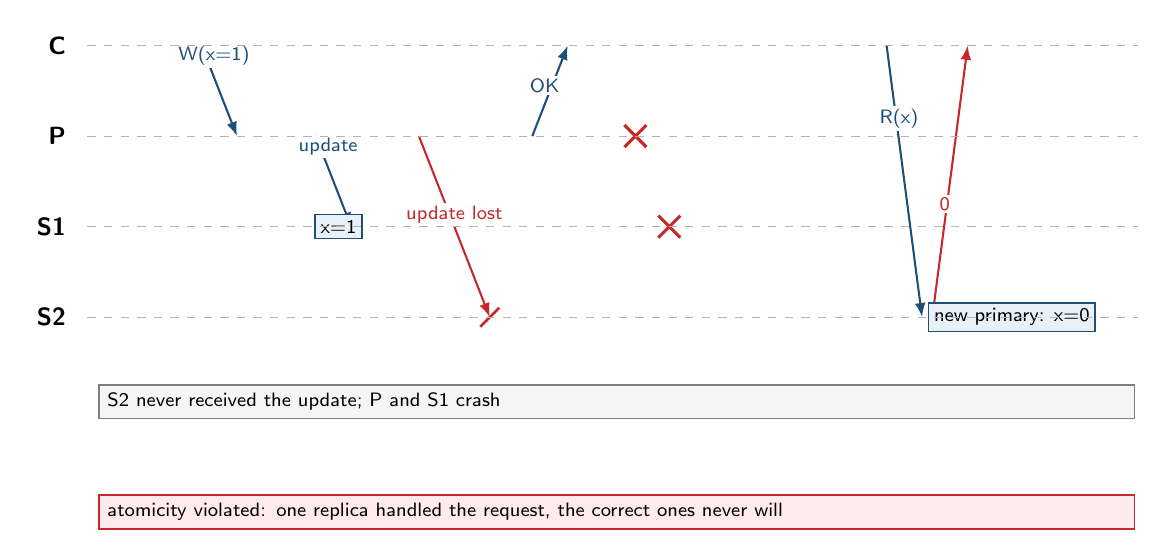
\begin{tikzpicture}[x=1cm,y=1cm]
\draw[-{Latex[length=1.8mm]},cblue,solid,line width=0.75pt] (1.45,0.000) -- (1.90,-1.150) node[pos=0.35,above,yshift=3pt,fill=white,inner sep=1pt,font=\scriptsize] {W(x=1)};
\draw[-{Latex[length=1.8mm]},cblue,solid,line width=0.75pt] (2.90,-1.150) -- (3.35,-2.300) node[pos=0.35,above,yshift=3pt,fill=white,inner sep=1pt,font=\scriptsize] {update};
\node[draw=cblue,fill=paleblue,line width=0.5pt,inner sep=2pt,font=\scriptsize,align=center] at (3.19,-2.300) {x=1};
\draw[-{Latex[length=1.8mm]},cred,line width=0.75pt] (4.21,-1.150) -- (5.11,-3.450) node[midway,above,fill=white,inner sep=1pt,font=\scriptsize] {update lost};
\draw[cred,line width=1pt] (4.99,-3.570) -- (5.23,-3.330);
\draw[-{Latex[length=1.8mm]},cblue,solid,line width=0.75pt] (5.65,-1.150) -- (6.10,0.000) node[pos=0.35,above,yshift=3pt,fill=white,inner sep=1pt,font=\scriptsize] {OK};
\draw[white,line width=1.6pt] (7.06,-1.150) -- (13.339999999999998,-1.150);
\draw[cred,line width=1.1pt] (6.82,-1.290) -- (7.10,-1.010);
\draw[cred,line width=1.1pt] (6.82,-1.010) -- (7.10,-1.290);
\draw[white,line width=1.6pt] (7.49,-2.300) -- (13.339999999999998,-2.300);
\draw[cred,line width=1.1pt] (7.25,-2.440) -- (7.53,-2.160);
\draw[cred,line width=1.1pt] (7.25,-2.160) -- (7.53,-2.440);
\node[anchor=north west,draw=cgrey,fill=palegrey,line width=0.5pt,inner sep=3pt,text width=12.939999999999998cm,align=left,font=\scriptsize] at (0.14,-4.300) {S2 never received the update; P and S1 crash};
\draw[-{Latex[length=1.8mm]},cblue,solid,line width=0.75pt] (10.15,0.000) -- (10.60,-3.450) node[pos=0.35,above,yshift=3pt,fill=white,inner sep=1pt,font=\scriptsize] {R(x)};
\draw[-{Latex[length=1.8mm]},cred,solid,line width=0.75pt] (10.73,-3.450) -- (11.18,0.000) node[pos=0.35,above,yshift=3pt,fill=white,inner sep=1pt,font=\scriptsize] {0};
\node[draw=cblue,fill=paleblue,line width=0.5pt,inner sep=2pt,font=\scriptsize,align=center] at (11.74,-3.450) {new primary: x=0};
\node[anchor=north west,draw=cred,fill=palered,line width=0.5pt,inner sep=3pt,text width=12.939999999999998cm,align=left,font=\scriptsize] at (0.14,-5.700) {atomicity violated: one replica handled the request, the correct ones never will};
\draw[cgrey!60,line width=0.4pt,dashed] (0,0.000) -- (13.339999999999998,0.000);
\node[anchor=east,font=\small\bfseries] at (-0.15,0.000) {C};
\draw[cgrey!60,line width=0.4pt,dashed] (0,-1.150) -- (13.339999999999998,-1.150);
\node[anchor=east,font=\small\bfseries] at (-0.15,-1.150) {P};
\draw[cgrey!60,line width=0.4pt,dashed] (0,-2.300) -- (13.339999999999998,-2.300);
\node[anchor=east,font=\small\bfseries] at (-0.15,-2.300) {S1};
\draw[cgrey!60,line width=0.4pt,dashed] (0,-3.450) -- (13.339999999999998,-3.450);
\node[anchor=east,font=\small\bfseries] at (-0.15,-3.450) {S2};
\end{tikzpicture}
\end{document}
